\documentclass{CInf_practice}

\sheet{7}{Schaltwerke}
\usepackage[gen]{eurosym}
\usetikzlibrary{automata,positioning,arrows.meta} 

\begin{document}
\cinftitle

\ex{Schaltwerksentwurf}{4 + 16 + 8 + 2 + 6 = 36}

\subex{Ein- \& Ausgaben}
\noindent Eingaben:
\begin{enumerate}[align=left,leftmargin=\marginparwidth]
   \item[$X_C$] 50 Cent einwerfen oder nicht
   \item[$X_E$] Euromünze einwerfen oder nicht
\end{enumerate}
Ausgaben:
\begin{enumerate}[align=left,leftmargin=\marginparwidth]
   \item[$Y_R$] 50 Cent auswerfen oder nicht
   \item[$X_G$] Getränk auswerfen oder nicht
\end{enumerate}

\subex{Zustandsgraph}

Es können nicht 2 Münzen gleichzeitig eingeworfen werden, die entsprechenden
Übergänge sind für Kongruenz mit der Tabelle dennoch aufgeführt.

Die Semantik der Zustände ist folgendermaßen:
\begin{ctabular}{ll}
   \hline
   Zustand & Semantik \\\hline
   A & Initial, wartend \\
   B & 1\euro{} fehlt \\
   C & 50 Cent fehlen \\
   D & Getränk ausgeben, kein Rückgeld\\
   E & Getränk ausgeben, Rückgeld ausgeben\\
   \hline
\end{ctabular}

\begin{center}
   \hspace{-2cm}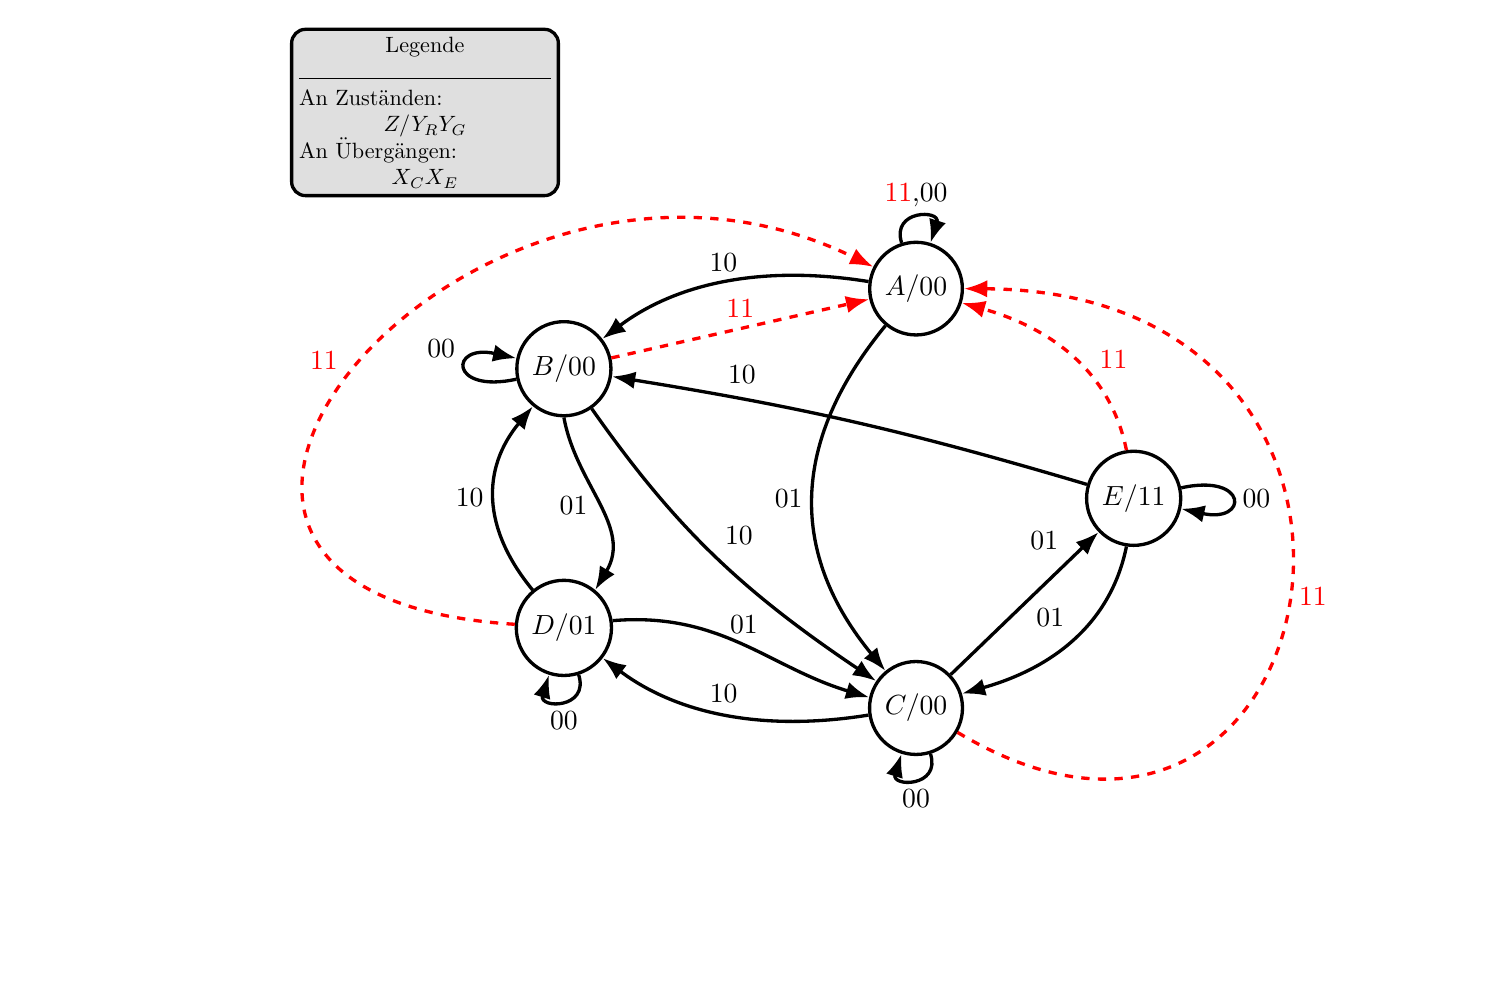
\begin{tikzpicture}[node distance=2cm,very thick,yscale=.7]
      \node[scale=.8,draw,rounded corners=5pt,fill=lightgray!50,text width=4cm] (legend) {
         \makebox[4cm]{Legende}\\
         \hrulefill \\
         An Zuständen: \makebox[4cm]{$Z/Y_R Y_G$} \\ An Übergängen: \makebox[4cm]{ $X_CX_E$ }
      };

      % math all nodes 
      \tikzset{state/.append style={execute at begin node=$, execute at end node=$}}

      \begin{scope}[xshift=5cm,yshift=-7cm]
         \foreach \n[count=\x] / \ausgabe in {A/00,B/00,D/01,C/00,E/11}{
            \node[state] at (\x*360/5:4cm) (\n) {\n/\ausgabe};
         }

         \tikzset{every loop/.style={looseness=5}}

         \path[-{Latex}] (A) edge[loop above] node {\textcolor{red}{11},00} ()
                         (A) edge[bend right] node[above] {10} (B)
                         (A) edge[bend right] node[left] {01} (C)
                         (B) edge[loop left] node[above left] {00} ()
                         (B) edge[draw=red,dashed] node[above] {\textcolor{red}{11}} (A)
                         (B) edge[bend left,out=0] node[left] {01} (D)
                         (B) edge[bend right=10] node[above right] {10} (C)
                         (D) edge[loop below] node[below] {00} ()
                         (D) edge[bend left] node[left] {10} (B)
                         (D) edge[bend left,in=180] node[above] {01} (C)
                         (C) edge[loop below] node[below] {00} ()
                         (C) edge[bend left] node[above] {10} (D)
                         (C) edge node[above left,pos=.8] {01} (E)
                         (E) edge[loop right] node[right] {00} ()
                         (E) edge[bend left] node[above left] {01} (C)
                         (E) edge[bend right=5] node[pos=.8,above right] {10} (B)
                         (E) edge[bend right,draw=red,dashed] node[right=5pt] {\textcolor{red}{11}} (A)

                         % long edges back to A
                         (D) edge[bend
                         left,draw=red,dashed,looseness=2,out=120,in=90]
                         node[left=5pt] {\textcolor{red}{11}} (A)
                         (C) edge[bend
                         right,draw=red,dashed,looseness=2,out=230,in=270]
                         node[right] {\textcolor{red}{11}} (A);
      \end{scope}
   \end{tikzpicture}
\end{center}

Der Graph ist offensichtlich konsistent und ``vollständig'', da für jede Eingabe
genau ein Ausgang pro Knoten existiert.

\subex{}

Wir haben 5 Zustände, weshalb 3 Bit zur Kodierung nötig sind.

\begin{ctabular}{ll}
   \hline
   Zustand & Kodierung \\\hline
   A & 000 \\
   B & 001 \\
   C & 010 \\
   D & 011 \\
   E & 100 \\
   \hline
\end{ctabular}

Die Zustandsübergangstabelle ist damit
\addtolength{\tabcolsep}{-3pt}
\begin{ctabular}{cccc|cc|cc|ccc}
   \hline
   Zustand & $Z_2^n$ & $Z_1^n$ & $Z_0^n$ & $X_C$ & $X_E$ & $Y_R$ & $Y_G$ &
   $Z_2^{n+1}$ & $Z_1^{n+1}$ & $Z_0^{n+1}$\\
   \hline\hline
   A & 0 & 0 & 0 & 0 & 0 & 0 & 0 & 0 & 0 & 0 \\
   A & 0 & 0 & 0 & 0 & 1 & 0 & 0 & 0 & 1 & 0 \\
   A & 0 & 0 & 0 & 1 & 0 & 0 & 0 & 0 & 0 & 1 \\
   A & 0 & 0 & 0 & 1 & 1 & 0 & 0 & X & X & X \\\hline

   B & 0 & 0 & 1 & 0 & 0 & 0 & 0 & 0 & 0 & 1 \\
   B & 0 & 0 & 1 & 0 & 1 & 0 & 0 & 0 & 1 & 1 \\
   B & 0 & 0 & 1 & 1 & 0 & 0 & 0 & 0 & 1 & 0 \\
   B & 0 & 0 & 1 & 1 & 1 & 0 & 0 & X & X & X \\\hline

   C & 0 & 1 & 0 & 0 & 0 & 0 & 0 & 0 & 1 & 0 \\
   C & 0 & 1 & 0 & 0 & 1 & 0 & 0 & 1 & 0 & 0 \\
   C & 0 & 1 & 0 & 1 & 0 & 0 & 0 & 0 & 1 & 1 \\
   C & 0 & 1 & 0 & 1 & 1 & 0 & 0 & X & X & X \\\hline

   D & 0 & 1 & 1 & 0 & 0 & 0 & 1 & 0 & 1 & 1 \\
   D & 0 & 1 & 1 & 0 & 1 & 0 & 1 & 0 & 1 & 0 \\
   D & 0 & 1 & 1 & 1 & 0 & 0 & 1 & 0 & 0 & 1 \\
   D & 0 & 1 & 1 & 1 & 1 & 0 & 1 & X & X & X \\\hline

   E & 1 & 0 & 0 & 0 & 0 & 1 & 1 & 1 & 0 & 0 \\
   E & 1 & 0 & 0 & 0 & 1 & 1 & 1 & 0 & 1 & 0 \\
   E & 1 & 0 & 0 & 1 & 0 & 1 & 1 & 0 & 0 & 1 \\
   E & 1 & 0 & 0 & 1 & 1 & 1 & 1 & X & X & X \\\hline

     & 1 & 0 & 1 & X & X & X & X & X & X & X \\
     & 1 & 1 & 0 & X & X & X & X & X & X & X \\
     & 1 & 1 & 1 & X & X & X & X & X & X & X \\\hline
\end{ctabular}
\addtolength{\tabcolsep}{3pt}

\subex{Minimierung}
Unter Ausnutzung der Don't-Cares minimieren sich die Ausgänge zu
\begin{eqnarray*}
   Y_R & = & Z_2^n \\
   Y_G & = & Z_2^n + Z_1^nZ_0^n
\end{eqnarray*}

\subex{Zustandstabelle D-Flipflops}
Da für D-Flipflops gilt $Q^{n+1} = D^n$, sind die Ansteuersignale genau die
Bits, die den Folgezustand codieren.

\addtolength{\tabcolsep}{-3pt}
\begin{ctabular}{cccc|cc|cc|ccc>{\columncolor{lightgray!50}}c>{\columncolor{lightgray!50}}c>{\columncolor{lightgray!50}}c}
   \hline
   Zustand & $Z_2^n$ & $Z_1^n$ & $Z_0^n$ & $X_C$ & $X_E$ & $Y_R$ & $Y_G$ &
   $Z_2^{n+1}$ & $Z_1^{n+1}$ & $Z_0^{n+1}$ & $D_2^n$ & $D_1^n$ & $D_0^n$ \\
   \hline\hline
   A & 0 & 0 & 0 & 0 & 0 & 0 & 0 & 0 & 0 & 0 & 0 & 0 & 0 \\
   A & 0 & 0 & 0 & 0 & 1 & 0 & 0 & 0 & 1 & 0 & 0 & 1 & 0 \\
   A & 0 & 0 & 0 & 1 & 0 & 0 & 0 & 0 & 0 & 1 & 0 & 0 & 1 \\
   A & 0 & 0 & 0 & 1 & 1 & 0 & 0 & X & X & X & X & X & X \\\hline

   B & 0 & 0 & 1 & 0 & 0 & 0 & 0 & 0 & 0 & 1 & 0 & 0 & 1 \\
   B & 0 & 0 & 1 & 0 & 1 & 0 & 0 & 0 & 1 & 1 & 0 & 1 & 1 \\
   B & 0 & 0 & 1 & 1 & 0 & 0 & 0 & 0 & 1 & 0 & 0 & 1 & 0 \\
   B & 0 & 0 & 1 & 1 & 1 & 0 & 0 & X & X & X & X & X & X \\\hline

   C & 0 & 1 & 0 & 0 & 0 & 0 & 0 & 0 & 1 & 0 & 0 & 1 & 0 \\
   C & 0 & 1 & 0 & 0 & 1 & 0 & 0 & 1 & 0 & 0 & 1 & 0 & 0 \\
   C & 0 & 1 & 0 & 1 & 0 & 0 & 0 & 0 & 1 & 1 & 0 & 0 & 1 \\
   C & 0 & 1 & 0 & 1 & 1 & 0 & 0 & X & X & X & X & X & X \\\hline

   D & 0 & 1 & 1 & 0 & 0 & 0 & 1 & 0 & 1 & 1 & 0 & 1 & 1 \\
   D & 0 & 1 & 1 & 0 & 1 & 0 & 1 & 0 & 1 & 0 & 0 & 1 & 0 \\
   D & 0 & 1 & 1 & 1 & 0 & 0 & 1 & 0 & 0 & 1 & 0 & 0 & 1 \\
   D & 0 & 1 & 1 & 1 & 1 & 0 & 1 & X & X & X & X & X & X \\\hline

   E & 1 & 0 & 0 & 0 & 0 & 1 & 1 & 1 & 0 & 0 & 1 & 0 & 0 \\
   E & 1 & 0 & 0 & 0 & 1 & 1 & 1 & 0 & 1 & 0 & 0 & 1 & 0 \\
   E & 1 & 0 & 0 & 1 & 0 & 1 & 1 & 0 & 0 & 1 & 0 & 0 & 1 \\
   E & 1 & 0 & 0 & 1 & 1 & 1 & 1 & X & X & X & X & X & X \\\hline

     & 1 & 0 & 1 & X & X & X & X & X & X & X & X & X & X \\
     & 1 & 1 & 0 & X & X & X & X & X & X & X & X & X & X \\
     & 1 & 1 & 1 & X & X & X & X & X & X & X & X & X & X \\\hline
\end{ctabular}

\ex{Schaltwerksminimierung}{2 + 4 + 9 + 9 + 4 = 28}
\subex{Automatentyp}
Da die Ausgaben allein von den Zuständen abhängig sind (Notation in den Zustandsknoten), handelt es sich um einen Moore-Automaten.

\subex{Zustandstabelle}
Wir verwenden X als Eingabe und Y als Ausgabe. 

\begin{ctabular}{c|c|ccc}
   \hline
   aktueller Zustand & aktuelle Ausgabe & \multicolumn{3}{c}{Folgezustand} \\
                     & Y                & X = & 0 & 1 \\ \hline
   A  & 0                &     & D & B \\
   B  & 0                &     & B & D \\
   C  & 0                &     & D & B \\
   D  & 1                &     & B & F \\
   E  & 1                &     & F & A \\
   F  & 1                &     & E & C \\
\end{ctabular}

\subex{Äquivalente Zustände: Tabelle}

\noindent\textbf{Gleiche Ausgabe}

Gruppen A-B-C und D-E-F

\noindent\bigskip\textbf{Folgezustände}

\begin{ctabular}{ll}
   Folgezustände Gruppe A-B-C: & D-B-D (für X = 0) \\
                               & B-D-B (für X = 1) \\
   Folgezustände Gruppe D-E-F: & B-F-E (für X = 0) \\
                               & F-A-C (für X = 1) \\
\end{ctabular}

\noindent\bigskip\textbf{Split}

Nach D-B-D bzw. B-D-B, aus denen D nicht in A-B-C vorkommt, muss A-B-C
aufgeteilt werden in A-C und B. Nach B-F-E muss D-E-F in D und E-F geteilt
werden.

Verbleibende Gruppen gleicher Ausgabe: A-C, B, D, E-F.

\noindent\bigskip\textbf{Folgezustände}

\begin{ctabular}{ll}
   Folgezustände Gruppe A-C:   & D-D (für X = 0) \\
                               & B-B (für X = 1) \\
   Folgezustände Gruppe B:     & B   (für X = 0) \\
                               & D   (für X = 1) \\
   Folgezustände Gruppe E-F:   & F-E (für X = 0) \\
                               & A-C (für X = 1) \\
   Folgezustände Gruppe D:     & B   (für X = 0) \\
                               & F   (für X = 1) \\
\end{ctabular}

\noindent\bigskip\textbf{Split}

Nach A-C (Folgezustand) muss E-F gesplittet werden. Da A-C (aktueller Zustand) erhalten bleibt, ergibt sich als Endergebnis:

\begin{ctabular}{c|c|ccc}
   \hline
   aktueller Zustand & aktuelle Ausgabe & \multicolumn{3}{c}{Folgezustand} \\
                     & Y                & X = & 0 & 1 \\ \hline
   A-C  & 0                &     & D & B \\
   B  & 0                &     & B & D \\
   D  & 1                &     & B & F \\
   E  & 1                &     & F & A-C \\
   F  & 1                &     & E & A-C \\
\end{ctabular}

\subex{Äquivalente Zustände: Implikationstafel}


\def\cell#1{\multicolumn{1}{|c|}{\begin{tabular}{c}#1\end{tabular}}}
\newcommand{\cancel}[1]{%
   \tikz[baseline=(tocancel.base)]{
      \node[inner sep=0pt,outer sep=0pt] (tocancel) {#1};
      \draw[red,thick] (tocancel.south west) -- (tocancel.north east);
   }%
}%
\newcommand{\Xout}{\cell{\huge X}% placeholder in case I am motivated to figure out
   % how to draw a cross (see: 
   % http://tex.stackexchange.com/questions/156162/strike-out-a-table-cell )
}

\begin{center}
   \begin{tabular}{cccccc}
      \cline{2-2}
      B & \cell{D-B\\B-D} &                  &         &                 &                 \\\cline{2-3}
      C & \cell{D-D\\B-B} & \cell{B-D\\D-B}  &         &                 &                 \\\cline{2-4}
      D & \Xout           & \Xout            & \Xout   &                 &                 \\\cline{2-5}
      E & \Xout           & \Xout            & \Xout   & \cell{B-F\\F-A} &                 \\\cline{2-6}
      F & \Xout           & \Xout            & \Xout   & \cell{B-E\\F-C} & \cell{F-E\\A-C} \\\cline{2-6}
        & A               & B                & C       & D               & E \\
   \end{tabular}

   \begin{tabular}{cccccc}
      \cline{2-2}
      B & \cell{\cancel{D-B}\\\cancel{B-D}} &                  &         &                 &                 \\\cline{2-3}
      C & \cell{D-D\\B-B} & \cell{B-D\\D-B}  &         &                 &                 \\\cline{2-4}
      D & \Xout           & \Xout            & \Xout   &                 &                 \\\cline{2-5}
      E & \Xout           & \Xout            & \Xout   & \cell{B-F\\F-A} &                 \\\cline{2-6}
      F & \Xout           & \Xout            & \Xout   & \cell{B-E\\F-C} & \cell{F-E\\A-C} \\\cline{2-6}
        & A               & B                & C       & D               & E \\
   \end{tabular}

   \begin{tabular}{cccccc}
      \cline{2-2}
      B & \Xout &                  &         &                 &                 \\\cline{2-3}
      C & \cell{D-D\\B-B} & \cell{\cancel{B-D}\\\cancel{D-B}}  &         &                 &                 \\\cline{2-4}
      D & \Xout           & \Xout            & \Xout   &                 &                 \\\cline{2-5}
      E & \Xout           & \Xout            & \Xout   & \cell{B-F\\F-A} &                 \\\cline{2-6}
      F & \Xout           & \Xout            & \Xout   & \cell{B-E\\F-C} & \cell{F-E\\A-C} \\\cline{2-6}
        & A               & B                & C       & D               & E \\
   \end{tabular}

   \begin{tabular}{cccccc}
      \cline{2-2}
      B & \Xout &                  &         &                 &                 \\\cline{2-3}
      C & \cell{D-D\\B-B} & \Xout  &         &                 &                 \\\cline{2-4}
      D & \Xout           & \Xout            & \Xout   &                 &                 \\\cline{2-5}
      E & \Xout           & \Xout            & \Xout   & \cell{\cancel{B-F}\\\cancel{F-A}} &                 \\\cline{2-6}
      F & \Xout           & \Xout            & \Xout   & \cell{\cancel{B-E}\\\cancel{F-C}} & \cell{F-E\\A-C} \\\cline{2-6}
        & A               & B                & C       & D               & E \\
   \end{tabular}

   \begin{tabular}{cccccc}
      \cline{2-2}
      B & \Xout &                  &         &                 &                 \\\cline{2-3}
      C & \cell{D-D\\B-B} & \Xout  &         &                 &                 \\\cline{2-4}
      D & \Xout           & \Xout            & \Xout   &                 &                 \\\cline{2-5}
      E & \Xout           & \Xout            & \Xout   & \Xout &                 \\\cline{2-6}
      F & \Xout           & \Xout            & \Xout   & \Xout & \cell{\cancel{F-E}\\\cancel{A-C}} \\\cline{2-6}
        & A               & B                & C       & D               & E \\
   \end{tabular}

   \begin{tabular}{cccccc}
      \cline{2-2}
      B & \Xout &                  &         &                 &                 \\\cline{2-3}
      C & \cell{D-D\\B-B} & \Xout  &         &                 &                 \\\cline{2-4}
      D & \Xout           & \Xout            & \Xout   &                 &                 \\\cline{2-5}
      E & \Xout           & \Xout            & \Xout   & \Xout &                 \\\cline{2-6}
      F & \Xout           & \Xout            & \Xout   & \Xout & \Xout \\\cline{2-6}
        & A               & B                & C       & D               & E \\
   \end{tabular}
\end{center}

Da D$\equiv$D und B$\equiv$B ist, ist auch A$\equiv$C. Wir erhalten erneut

\smallskip

\begin{ctabular}{c|c|ccc}
   \hline
   aktueller Zustand & aktuelle Ausgabe & \multicolumn{3}{c}{Folgezustand} \\
                     & Y                & X = & 0 & 1 \\ \hline
   A-C  & 0                &     & D & B \\
   B  & 0                &     & B & D \\
   D  & 1                &     & B & F \\
   E  & 1                &     & F & A-C \\
   F  & 1                &     & E & A-C \\
\end{ctabular}

\subex{Minimierter Zustandsgraph}
A-C wird nur als A bezeichnet!

\begin{center}
   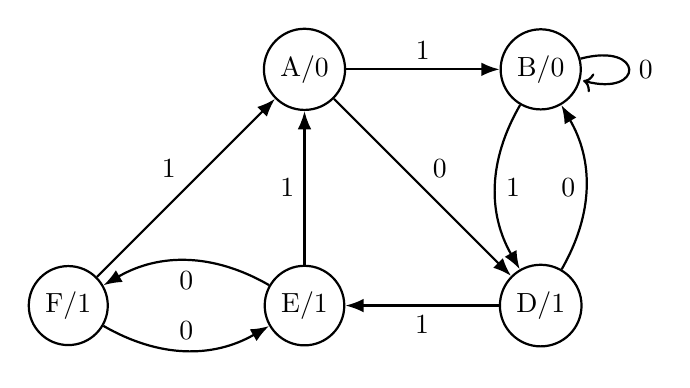
\begin{tikzpicture}[node distance=3cm,thick]
      \node[state] (A)              {A/0};
      \node[state] (B) [right of=A] {B/0};
      \node[state] (D) [below of=B] {D/1};
      \node[state] (F) [below of=A] {E/1};
      \node[state] (E) [left of=F]  {F/1};

      \path[-{Latex}] (A) edge             node[above right] {0} (D)
      (A) edge             node[above]       {1} (B)
      (B) edge[loop right] node[right]       {0} (B)
      (B) edge[bend right] node[right]       {1} (D)
      (D) edge[bend right] node[left]        {0} (B)
      (D) edge             node[below]       {1} (F)
      (E) edge[bend right] node[above]       {0} (F)
      (E) edge             node[above left]  {1} (A)
      (F) edge[bend right] node[below]       {0} (E)
      (F) edge             node[left]        {1} (A)
      ;
   \end{tikzpicture}
\end{center}

\ex{Schaltwerksanalyse}{3 + 7 + 8 + 6 + 4 + 8 = 36}

\subex{}

Der Automat ist ein Mealy-Automat, da es einen Weg vom Eingang zum Ausgang gibt,
der nicht durch eines der Flipflops läuft. Zwar ist es an sich aufgrund der
getatkteten Flipflops synchron, da es ein Mealy-Automat ist, können aber
Eingaben asynchron am Ausgang sichtbar sein. Da Eingaben vorhanden sind, ist der
Automat nicht autonom. Ein Aufzug, der nicht auf Eingaben reagiert wäre auch
eher sinnlos bis gefährlich.

\subex{}

Die Ansteuersgleichungen sind
\begin{IEEEeqnarray*}{rCl}
   T_1 & = & X^n\comp{Z_1^n}Z_0^n \\
   T_0 & = & X^n\comp{Z_0^n} + \comp{Z_1^n}Z_0^n + \comp{X^n} Z_1^n
\end{IEEEeqnarray*}

Für die Ausgänge gilt
\begin{IEEEeqnarray*}{rCl}
   Y_R & = & X^n \\
   Y_M & = & X^n\comp{Z_0^n} + \comp{Z_1^n}Z_0^n + \comp{X^n}Z_1^n = T_0
\end{IEEEeqnarray*}

\subex{}

\begin{ctabular}{ccc|cc|cc|cc|cc}
   $Z_1^n$ & $Z_0^n$ & $X$ & $T_1$ & $T_0$ & $Z_1^{n+1}$ & $Z_0^{n+1}$ & $D_1$ &
   $D_0$ & $Y_R$ & $Y_M$ \\\hline\hline
   0 & 0 & 0 & 0 & 0 & 0 & 0 &   &   & 0 & 0 \\
   0 & 0 & 1 & 0 & 1 & 0 & 1 &   &   & 1 & 1 \\
   0 & 1 & 0 & 1 & 1 & 0 & 0 &   &   & 0 & 1 \\
   0 & 1 & 1 & 1 & 1 & 1 & 0 &   &   & 1 & 1 \\

   1 & 0 & 0 & 0 & 1 & 0 & 1 &   &   & 0 & 1 \\
   1 & 0 & 1 & 0 & 1 & 1 & 1 &   &   & 1 & 1 \\
   1 & 1 & 0 & 0 & 1 & 1 & 0 &   &   & 0 & 1 \\
   1 & 1 & 1 & 0 & 0 & 1 & 1 &   &   & 1 & 0 \\
\end{ctabular}

Es folgen die Übergangsgleichungen 
\begin{IEEEeqnarray*}{rCl}
   Z_1^{n+1} & = & Z_1^n Z_0^n + X^n Z_0^n + X^n Z_1^n \\
Z_0^{n+1} & = & Z_1^n \comp{Z_0^n} + X^n\comp{Z_0^n} + X\comp{Z_1^n}
\end{IEEEeqnarray*}

\begin{center}
   \hspace{-2cm}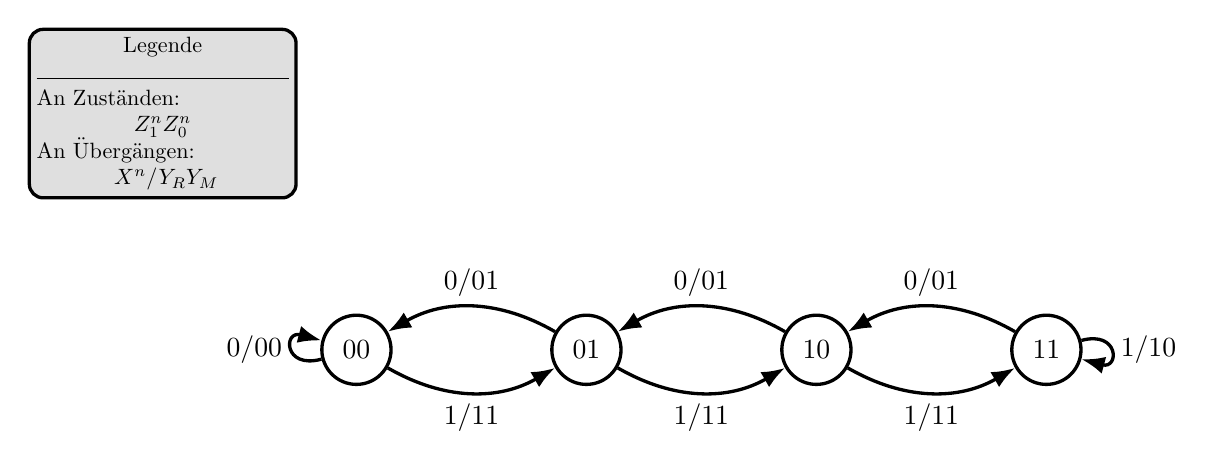
\begin{tikzpicture}[node distance=2cm,very thick]
      \node[scale=.8,draw,rounded corners=5pt,fill=lightgray!50,text width=4cm] (legend) {
         \makebox[4cm]{Legende}\\
         \hrulefill \\
         An Zuständen: \makebox[4cm]{$Z_1^n Z_0^n$} \\ An Übergängen:
         \makebox[4cm]{ $X^n/Y_R Y_M$}
      };

      % math all nodes 
      \tikzset{state/.append style={execute at begin node=$, execute at end node=$}}

      \begin{scope}[yshift=-3cm]

         \tikzset{every loop/.style={looseness=5}}

         \foreach \x / \y / \z in {A/00/{(0,0)},B/01/A,C/10/B,D/11/C}{
            \node[state,right=of \z] (\x) {\y};
         }

         \path[-{Latex}] (A) edge[loop left] node[left] {0/00} ()
         (A) edge[bend right] node[below] {1/11} (B)
         (B) edge[bend right] node[below] {1/11} (C)
         (C) edge[bend right] node[below] {1/11} (D)
         (D) edge[loop right] node[right] {1/10} ()
         (D) edge[bend right] node[above] {0/01} (C)
         (C) edge[bend right] node[above] {0/01} (B)
         (B) edge[bend right] node[above] {0/01} (A)
         ;
      \end{scope}
   \end{tikzpicture}
\end{center}

Das Schaltwerk steuert einen Aufzug, also is $X$ vermutlich die Fahrtrichtung
und $Y_R$ gibt an, in welche Richtung sich die Maschinerie entsprechend dreht,
währen $Y_M$ angibt, \emph{ob} sie sich dreht (man kann ganz oben nicht weiter
hoch fahren und ganz unten nicht weiter runter). Die Zustände repräsentieren
Stockwerke.
\end{document}
